\setchapterpreamble[u]{%
  \margintoc\hfil
  \dictum[Richard Feynman]{What I cannot create,\\I do not understand.}
}

\chapter{Methods}
\labch{methods}
% Write in theorem-proof fashion

The following sections describe the design and build process --- including the reasoning behind the decisions taken --- of the magnETHical NMR spectrometer. \reffig{block-diagram} shows an overview schematic of the main components that will be discussed.

\begin{figure}[hbt]
  \centering
  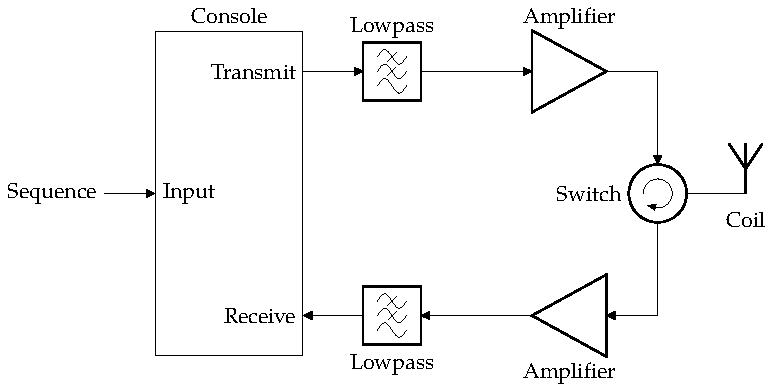
\includegraphics{block_diagram.pdf}
  \caption{\captiontitle{Block Diagram.} The main components of the magnETHical NMR spectrometer, including Console, Lowpass filters, analog amplifiers, transmit-receive switch and transmit-receive coil.}
  \labfig{nmr_citations}
\end{figure}

\section{The console}
\begin{marginfigure}
  \centering
  \includesvg{simple_pulse_sequence.svg}
  \caption{\captiontitle{Simple pulse sequence} The usual depiction of a simple pulse sequence. The \enquote{RF pulse} is a high frequency \acrshort{rf} pulse close to the resonance frequency of the nuclei to be observed. After the pulse, a decaying sinus signal can be received on the same coil -  the so-called \acrfull{fid}.}
  \labfig{simple-pulse-sequence}
\end{marginfigure}


building of the amplifiers
building of the switch
building the coil
building the power supply

\chapter{Building process}
\labch{building-process}

\chapter{Lessons learned}
\labch{lessons-learned}